\section{Object diffusion mini-protocol}%
\label{sec:object-diffusion-protocol}

\definecolor{mygreen}{rgb}{0.109804,0.698039,0.341176}
\definecolor{myblue}{rgb}{0.360784,0.423529,255}

\usetikzlibrary{automata, positioning, arrows}
\usetikzlibrary{arrows,calc,matrix,shapes}

\tikzset{
    state/.style={
           rectangle,
           rounded corners,
           draw=black, very thick,
           minimum height=2em,
           inner sep=2pt,
           text centered,
           },
}

\newcommand{\header}[1]{\textbf{#1}}

\newcommand{\state}[1]{\texttt{#1}}
\newcommand{\trans}[1]{\texttt{#1}}
\newcommand{\msg}[1]{\textbf{\texttt{#1}}}

\newcommand{\StInit}             {\state{StInit}}
\newcommand{\StIdle}{\state{StIdle}}
\newcommand{\StDone}{\state{StDone}}
\newcommand{\StObjIdsBlocking}    {\state{StObjIds Blocking}}
\newcommand{\StObjIdsNonBlocking} {\state{StObjIds NonBlocking}}
\newcommand{\StObjs}              {\state{StObjs}}

\newcommand{\MsgInit}            {\msg{MsgInit}}
\newcommand{\MsgRequestObjIdsNB}  {\msg{MsgReqObjIds NonBlocking}}
\newcommand{\MsgRequestObjIdsB}   {\msg{MsgReqObjIds Blocking}}
\newcommand{\MsgReplyObjIds}      {\msg{MsgReplyObjIds}}
\newcommand{\MsgRequestObjs}      {\msg{MsgReqObjs}}
\newcommand{\MsgReplyObjs}        {\msg{MsgReplyObjs}}
\newcommand{\MsgDone}{\msg{MsgDone}}
\newcommand{\MsgServerIdle} {\msg{MsgServerIdle}}

\begin{figure}[h]
  \begin{center}
    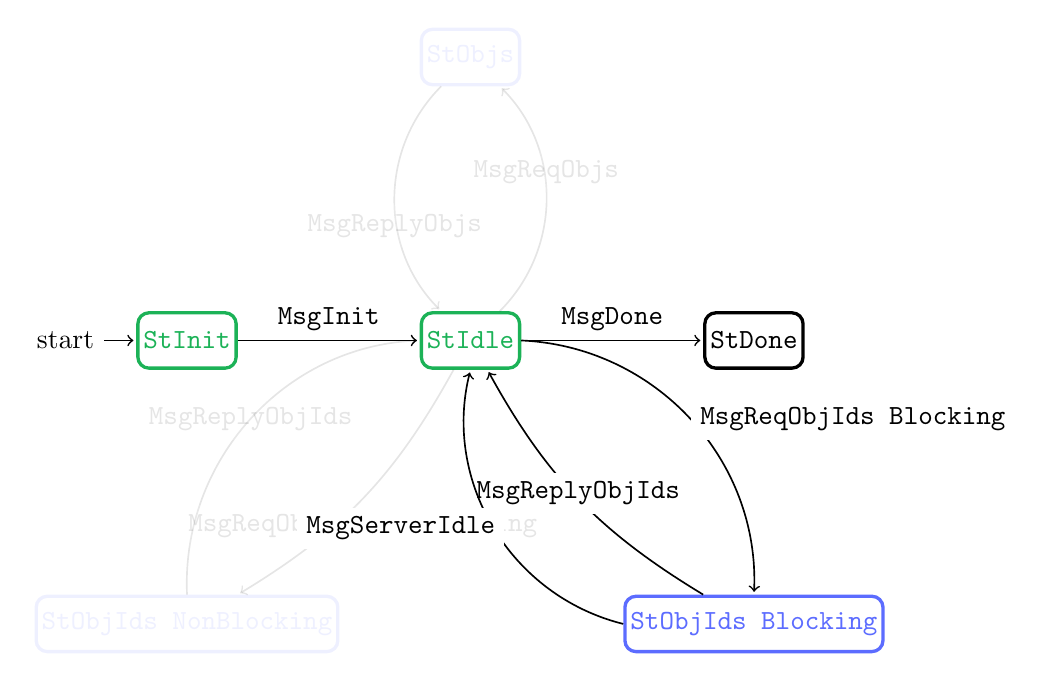
\begin{tikzpicture}[->,shorten >=1pt,auto,node distance=4.5cm, semithick, scale=0.9]
      \tikzstyle{every state}=[fill=red,draw=none,text=white]
      \node[state, mygreen, initial] (I) at (-4,  0) {\StInit};
      \node[state, mygreen]           (A) at ( 0,  0) {\StIdle};
      \node[state]                   (B) at (4, 0) {\StDone};
      \node[state, myblue]          (C) at ( 4, -4) {\StObjIdsBlocking};
      \node[state, myblue, opacity=0.1]          (D) at (-4, -4) {\StObjIdsNonBlocking};
      \node[state, myblue, opacity=0.1]          (E) at ( 0,  4) {\StObjs};
      \draw[opacity=0.1] (D)  edge[bend left=45]      node[fill = white, anchor = center]{\MsgReplyObjIds}                  (A);
      \draw[opacity=0.1] (A)  edge[bend left=15]      node[fill = white, below = 2pt]{\MsgRequestObjIdsNB} (D);
      \draw[opacity=0.1] (A)  edge[bend right=45]      node[fill = white, above = 2pt]{\MsgRequestObjs}     (E);
      \draw[opacity=0.1] (E)  edge[bend right=45]      node[fill = white, below = 2pt]{\MsgReplyObjs}       (A);
      \draw (I)  edge                    node[above]{\MsgInit}                                                 (A);
      \draw (A)  edge                    node[above]{\MsgDone}                                                 (B);
      \draw (A)  edge[bend left=45]       node[fill = white, anchor = west]{\MsgRequestObjIdsB}  (C);
      \draw (C)  edge[bend left=15]      node[fill = white, above = -6pt]{\MsgReplyObjIds}     (A);
      \draw (C)  edge[bend left=45]      node[fill = white, left = -4pt]{\MsgServerIdle}     (A);
    \end{tikzpicture}
  \end{center}
  \caption{Object diffusion state machine}%
  \label{fig:object-diffusion-state-machine}
\end{figure}

\newcommand\argfont[1]{\textbf{\texttt{\textit{#1}}}}
